\documentclass[bare_jrnl_transmag]{subfiles}
\begin{document}

\subsection{Data Collection}

The data was collected using the dataset from the paper "Are We Ready for Autonomous Drone Racing?
The UZH-FPV Drone Racing Dataset" \cite{Delmerico19icra}. The paper contains 27 different flight paths with camera data, inertial and ground truth positioning to set up robust pose and position tracking algorithms. \newline

The data was collected by flying a small FPV drone around various different indoor and outdoor paths, recording the pertinent data mentioned above. The FPV drone used by the team contained measurements from a stereo camera, an IMU and a reflector (for tracking ground truth). Figure  \ref{fig:drone_setup} shows the setup of the physical drone.

\begin{figure}[H]
    \centering
    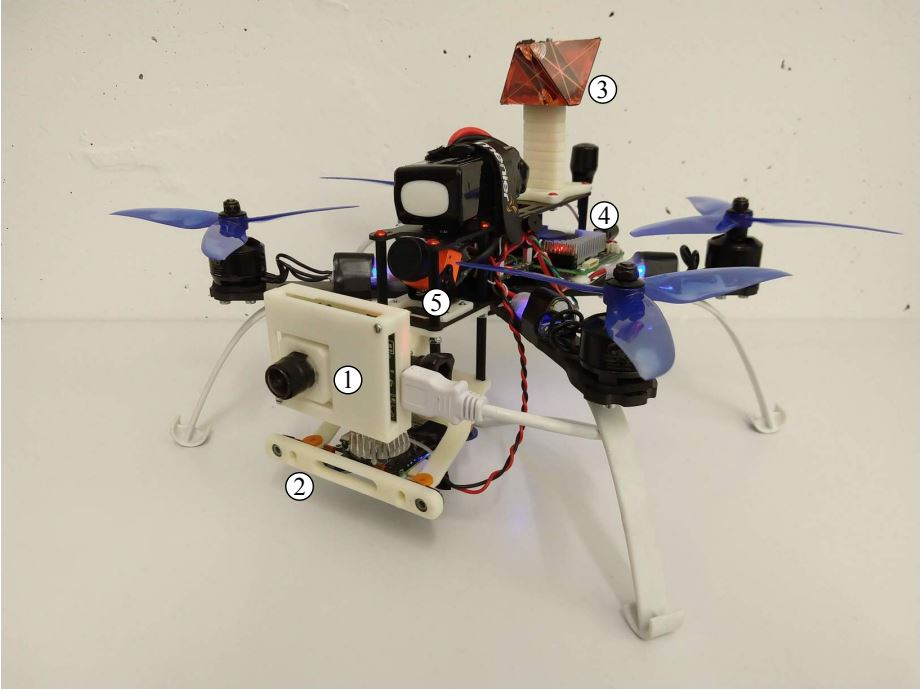
\includegraphics[width=0.8\linewidth]{figures/drone_setup.jpg}
    \caption{Drone Measurement Setup. : 
    1 mDAVIS 2 Snapdragon Flight with fisheye stereo cameras 3 Omnidirectional reflector that provides the ground truth position. 4 Up Board
    used for recording the DAVIS data. 5 FPV camera used by the human pilot \cite{Delmerico19icra}}
    \label{fig:drone_setup}
\end{figure}

For visual-inertial odometry (VIO), only the camera and IMU are essential; the reflector is used solely for obtaining ground truth. A key part of the implementation involves transforming between coordinate frames—specifically from the camera and IMU frames to the world frame. Since the IMU and drone have different axes, and the drone’s orientation changes as it moves, a rotation is required to align the IMU frame with the drone frame. The Madgwick filter was used to estimate the drone’s pose in the world frame. Additional transformations were applied to relate the camera frame to both the drone and world frames. Figure \ref{fig:drone_axis} illustrates the different reference axes of the onboard sensors

\begin{figure}[H]
    \centering
    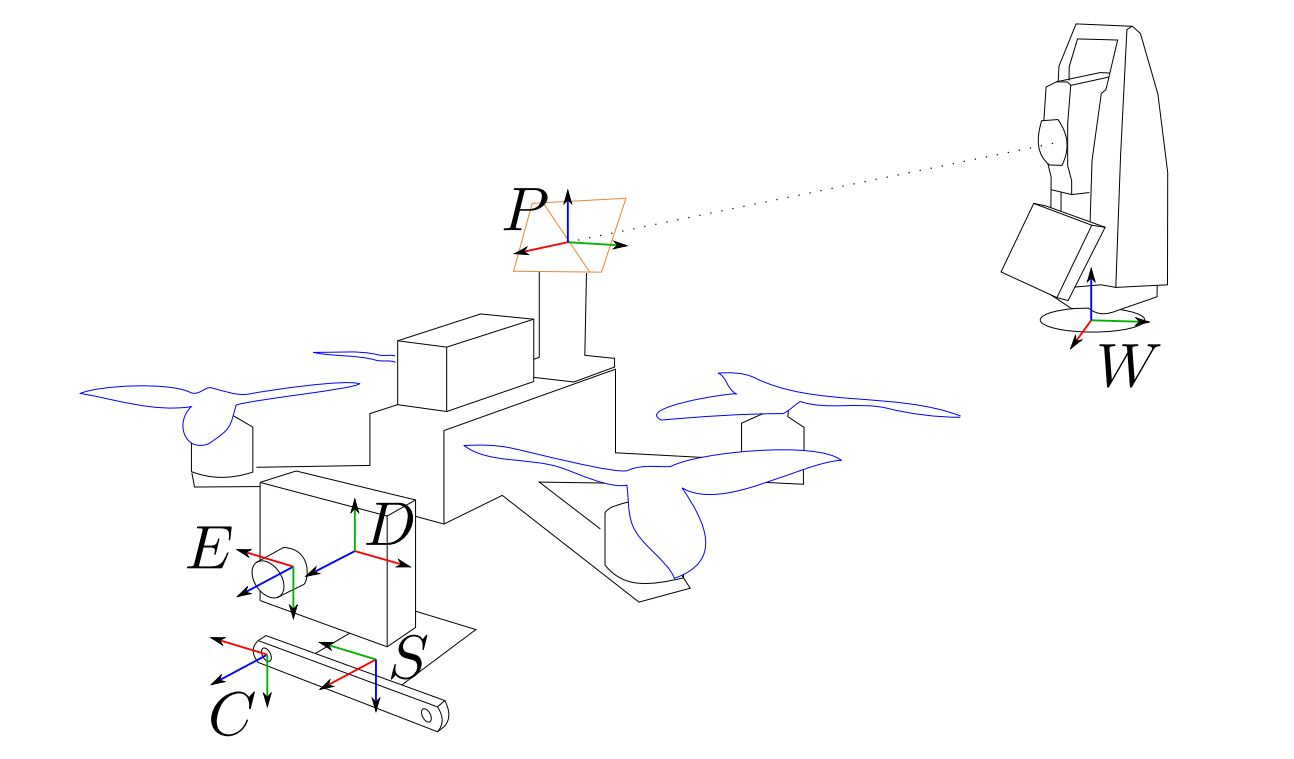
\includegraphics[width=0.8\linewidth]{figures/drone_axis.jpg}
    \caption{Drone Axis: C: Camera Frame, S: IMU Frame, P: Reflector Frame/Drone Frame, W: World Frame \cite{Delmerico19icra}}
    \label{fig:drone_axis}
    
\end{figure}

\end{document}